\chapter{相关技术背景及算法}
\label{chap:algorithm}

\begin{figure}[ht]
\centering
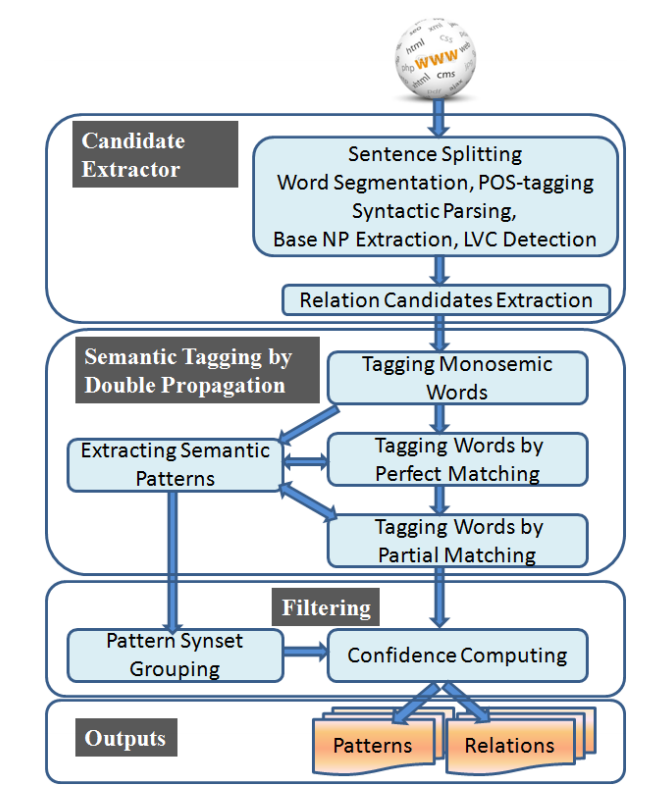
\includegraphics[width=10cm]{ZORE}
\caption{ZORE 体系结构}\label{fig:ZORE}
\end{figure}

\section{ZORE 的简介}
ZORE 的体系结构如图 ~\ref{fig:ZORE} 所示。它由三个部件组成。第一个部件是候选关系提取器,这个提取器获取输入的文本然后进行句子的分割、字词的分割、添加 POS 标签、句法解析、基本的 NP(noun phrase,名词短语) 提取、轻量化的动词结构(LVC,light verb structure)探测和候选关系提取。它的输出是所有候选关系的集合。第二个部件对关系进行添加标签,然后通过双重拓展算法提取语义模式。第三个部件则将被提取出的模式进行同义词集分组,关系则依据“可信分数”进行过滤。

\subsection{提取候选关系}

\subsubsection{解析与基本的 NP 提取}
ZORE 通过应用一系列的 NLP(Natural Language Process,自然语言处理)工具对输入的文本进行流水线处理来分析句法结构。每个句子都通过 Stanford 分割器\citep{chang2008}被分割为一个字词列表,并通过 ZPar \citep{zhang2011}来进行解析,通过标准 CTB \citep{xue2005}来添加 POS 标志和分析结构组成。并对最后生成的构成树使用 Stanford 解析器\citep{chang2008}将其变形为有 Stanford dependencies 的投影树。

接下去,基本的 NPs (名词短语)从依赖树中被提取出来,在这里基本 NP 是一个最大短语,其字词只能拥有来自表 ~\ref{tab:NP} 第一行的 POS。基本 NP 的核心词语可以是一个名词,一个代词,一个数字或是一个量词(表 ~\ref{tab:NP} 的第二行)。基本 NP 里的依赖标签只能来自表 ~\ref{tab:NP} 的第三行。所以,很明显的,一个基本 NP 并不包含其他的基本 NP,并且它本身也不被其他的基本 NP 所包含。

\begin{longtable}{cc}
% 首页表头
\caption[基本 NP 标志表]{包含了 POS 标志和依赖标签,在前三行的标签被用来进行基本 NP 的提取,而最后一行中的标签用于从基本 NP 遍历到谓词短语} \label{tab:NP} \\
\toprule[1.5pt]
  & 标志\\
\midrule[1pt]
\endfirsthead
% 续页表头
\caption[]{(续)} \\
\toprule[1.5pt]
  & 标志\\
\midrule[1pt]
\endhead
% 首页表尾
\hline
\multicolumn{2}{r}{\small 续下页}
\endfoot
% 续页表尾
\bottomrule[1.5pt]
\endlastfoot
基本 NP 修饰语   &   NN (common noun), M (measure word), \\
    &   CD (cardinal number), OD (ordinal number),\\
    &   PN (pronoun), NR(proper noun),\\
    &   NT (temporal noun), \\
    &   JJ (other noun-modifier), or PU (punctuation) \\
    \hline
基本 NP 中的标签  &   nn (noun compound modifier), conj (conjunct),\\
    &   nummod (number modifier),\\
    &   cc (coordinating conjunction),\\
    &   clf (classifier modifier), det (determiner),\\
    &   ordmod (ordinal number modifier),\\
    &   punct (punctuation),\\
    &   dep (other dependencies),\\
    &   or amod (adjectival modifier) \\
    \hline
基本 NP 核心    &   NN (common noun), M (measure word), \\
    &   CD (cardinal number), OD (ordinal number),\\
    &   PN (pronoun), NR(proper noun),\\
    &   NT (temporal noun) \\
    \hline
基本 NP 到谓词的过渡标签  &   nsubj (nominal subject), conj (conjunct),\\
    &   dobj (direct object), advmod (adverbial modifier),\\
    &   prep (preposi-tional modifier),\\
    &   pobj (prepositional object), lobj (localizer object),\\
    &   range (dative object that is a quantifierphrase),\\
    &   tmod (temporal modifier),\\
    &   plmod (localizer modifier of a preposition),\\
    &   attr (attributive), loc (local-izer),\\
    &   top (topic), xsubj (controlling subject),\\
    &   ba (“ba” construction),\\
    &   nsubjpass (nominal passive subject) \\
\end{longtable}

\subsubsection{探测轻量化动词结构}
在语言学中,“轻量化动词”(LVC,light verb construction)指的是一个本身几乎没有语义的动词,并且通常都是和一个名词形成一个谓语\citep{Etzioni2011}。例如,有着“轻量化动词结构”的谓语包括“是国家的”和“宣称拥有主权”,他们的轻量化动词分别是“是”和“宣称”。对 LVC 不合适的处理可能由于不详细的提取导致出现很明显的问题。例如,如果之前两个句子“是国家的”和“宣称拥有主权”中的“是”和“宣称”被作为谓语提取,就会导致提取出的关系无法让人显式地获得有用的信息\citep{Etzioni2011},例如(“税收是国家的收入来源。”,提取出的关系可能是(税收,是,收入来源))。重构动词(ReVerb\citep{Etzioni2011})则解决了以上的问题,通过严格的句法限制让处于动词短语(例如“是”)和介词(例如“的”)中间的名词短语(例如“国家”)被认为是谓词短语的一部分而不是一个参数,从而得出了(税收,是国家的,收入来源)这个关系。

在中文语境中,LVCs 出现的频率非常高,并且应该被妥善地处理,从而保证被提取出的关系可以提供有用的信息。在中文语境中,介词扮演着动词的修饰语,并且可以在动词的左边或右边。例如图 ~\ref{fig:sentence1} 中的例句“侯建国校长就职于中国科学技术大学。”可以被改写为“侯建国校长于中国科学技术大学就职。”,而这两个句子中的介词“于”则分别位于谓词短语“就职”的右边和左边。

中文的 LVCs 可以被归为两类,即“伪 LVC”和“平凡 LVC”。对于伪 LVC,谓词是一个“假的动词”,例如“进行”和“给予”,都是有着名词短语作为他们的对象。因为中文的“假的动词”是一个闭集,我们通过寻找来自语料库的“假的动词”进行探测这种伪 LVC。而对于平凡 LVC,它的谓词则是平凡的动词,即它的谓词有着正常的结构或一个平凡的名词作为对象。例如,“展开调查”就是这种平凡 LVC。


\begin{longtable}{cc}
% 首页表头
\caption[伪 LVC 与平凡 LVC 样例表]{伪 LVC(*) 与平凡 LVC (**)样例表,左列的动词和右列的名词组合生成 LVC,并作为谓词短语。} \label{tab:LVC} \\
\toprule[1.5pt]
动词 & 名词\\
\midrule[1pt]
\endfirsthead
% 续页表头
\caption[]{(续)} \\
\toprule[1.5pt]
动词 & 名词\\
\midrule[1pt]
\endhead
% 首页表尾
\hline
\multicolumn{2}{r}{\small 续下页}
\endfoot
% 续页表尾
\bottomrule[1.5pt]
\endlastfoot
进行(*)   &   发行,分析,收集,修改,访问,处罚\\
    \hline
有(*)  &   影响,贡献,兴趣,帮助,认识,期望\\
    \hline
产生(**)    &   影响,兴趣,怀疑,冲击,好感,恐惧\\
    \hline
造成(**)  &   影响,破坏,伤害,威胁,压力,干扰\\
    \hline
表示(**)  &   满意,欢迎,尊重,担忧,哀悼,感谢\\
    \hline
展开(**)  &   调查,攻击,攻势,批评,批判,诉讼\\
\end{longtable}

平凡 LVC 比伪 LVC 更加难以探测,我们通过上下文的语境来对平凡 LVC 进行探测。包括在 LVC 里的 NP 本身,一个平凡 LVC 通常控制着两个 NP,而处在后面的 NP 则通过一个与 LVC 有关的介词来联系在一起,例如“对,对于,针对,向,同,与,和”。基于以上的现象,一个通用的方法来鉴别平凡 LVC 产生了,即通过寻找在大型语料库中频繁地与 LVC 相关的介词一起出现,被自动解析的动词对象结构。对于一个给定的动词对象 v,用 $f^v$ 和 $f^p$ 分别表示 v 出现的频率和与 v 一起出现的与 LVC 有关的介词的频率。定义 v 成为 LVC 的统计强度为 $f^p / f^v$。如果 v 的统计强度达到了 $t^{lvc}$ 的阈值,则将 v 定义为 LVC。表 ~\ref{tab:LVC} 描述了一些高频率出现的 LVC,通过这种方式被自动提取出来。

\subsubsection{提取候选关系}
ZORE 尝试从含有两个或更多基本 NP 的句子里抽取候选关系。对于给定的两个基本 NP,我们遍历依赖树来获取连结他们的最短路径。而这个最短路径可以仅仅包括表 ~\ref{tab:NP} 中第四行的依赖标志,并且必须包括至少一个来自“nsubj”和“dobj”的标志,从而保证这个谓词短语被包括在最短路径中。如果获取到了这样的最短路径,则其他的被同一个谓词短语所控制的基本 NP 也被包括进了这个目标关系里,得出一个 n 元的候选关系,当中的每个基本 NP 都对应着一个参数。依据这个谓词短语,候选关系可以被归为以下几类:

\newtheorem*{CDLR}{平凡与伪 LVC 关系}
\begin{CDLR}
    在这种关系里,最短路径的谓词短语是一个 LVC(例如一个轻量动词和一个普通的对象)。那两个基本的 NP 可以是轻量动词的前置词或子词。以“老李对我的学业有很大帮助”作为例句,“有”和“帮助”结合形成了一个平凡 LVC,并被当成了一个谓词短语,从而得出了关系(老李,Pred[有帮助],我的学业)。
\end{CDLR}
\newtheorem*{VR}{动词关系}
\begin{VR}
    在这种关系里,一个动词则作为一个谓词短语。例如,这个关系(侯建国校长,Pred[就职],中国科学技术大学)提取自图 ~ref{fig:sentence1} 则是一个典型的动词关系。
\end{VR}
\newtheorem*{RCR}{关联从句关系}
\begin{RCR}
    在这种关系里,核心词语是一个名词,被一个关联从句所修饰,并在语义上作为这个关联从句的谓词的参数。“就职于中国科学技术大学的侯建国校长。”这个句子是图 ~\ref{fig:sentence1} 的一个同义句,有着一样的谓词短语和参数。然而,从这个句子里提取出的关系是一个关联从句关系(Pred[就职],中国科学技术大学,侯建国校长),和图 ~\ref{fig:sentence1} 句子的关系属于一样的模式同义词集。
\end{RCR}

\subsection{双重拓展的语义标注}
基本思想是通过进行对候选关系的参数的核心词语进行词语义标注,迭代地识别关系和模式。对于给定的候选关系集合和语义分类系统,进行拓展包括三个步骤。第一步,候选关系中的单义参数会被用语义类别标注,例如 Af 和 Di,从而获取语义模式。在第二步和第三部,未被标注的的含义模糊和未知词将会分别通过完全匹配和部分匹配进行标注。在每一步的末尾,语义模式来自被提取出和被标注过的关系的概括,之后语义模式被用来帮助下一步的关系标注。因为这种双向的信息交换,这种方式被称之为“双重拓展”。

\subsubsection{第一步:标注单义的参数}
每个在候选关系内的参数都是基本 NP,因为基本 NP 都是向心结构的\citep{endocentric2017},所以我们可以将一个基本 NP 的核心词语语义类别当作这个基本 NP 的语义类别。在一个分类系统里,每个字词都和一个或更多的语义类别有关。然而,在这步里,只有单义的词语才会被标注,而词义模糊和未知的词语都会被忽略,不会被标注。

大部分被命名的实体并没有被包括在分类系统中。然而,在标注了 POS 标签后,大部分的已命名实体将会被探测为 NR(proper noun,专有名词)。而这导致那些已命名的实体将会被作为词义模糊的词语处理,可以是人名,组织名,或地名。未被分类系统包括的已命名实体将会在第二、三步里被标注。

在这步之后,在一些候选关系里的所有参数都已经被用语义分类标注。这些候选关系被称为“已标注候选关系”,而其他的候选关系则被称之为“未标注候选关系”。已标注候选关系将会被归纳为语义模式,包括句法模式和语义标签,就像图 ~\ref{fig:sentence1} 里所描述的。将由此生成的语义模式称之为$Set^{SemPat}$

\subsubsection{第二步:完全的模式匹配标注}
在这步,将会通过语义模式匹配对未标注候选关系里的参数进行标注。对于给定的未标注候选关系 r,我们对每一个有着模糊词义的核心词语,获取一个潜在语义类型集合。对于有着未知核心词语的参数,我们根据他们的单字获取潜在语义类型集合。98\% 的中文字词至少都有一个同义字词\citep{qiu2011},并且原字词和同义字词之间至少有一个字一样。对于中文名词,同义字词的集合通常也有着至少一或二个一样的字。所以,对于获取未知字词的潜在的词义类型策略就大致成型了。

首先,对于给定的未知字词 $w^u$,如果我们可以发现一个已知的字词 $w^k$ 与未知的字词 $w^u$ 结尾的两个字一样,则 $w^k$ 的语义类型会被作为 $w^u$ 的潜在语义类型。否则,如果 $w^u$ 和 $w^k$ 最后一个字都一样,那么 $w^k$ 的语义类型会被作为 $w^u$ 的潜在语义类型。

接下去我们开始获取未标注的候选关系的潜在语义标签,这里的未标注候选关系的所有参数已经被潜在语义类型所标注。就像第一步里的,我们将关系 $r$ 归纳为一个句法模式 $pat^{syn}$,之后将 $pat^{syn}$ 与每一个 $r$ 的潜在语义标签来生成潜在语义模式。为了避免一个或更多 $r$ 的潜在语义模式存在于 $Set^{SemPat}$ 中,如果那些语义模式当中频率最高的模式超过了阈值 $t^{sem}$ ,那么符合条件的模式将会被作为 $r$ 的语义模式,由此我们推断 $r$ 的语义标志和之后 $r$ 的每个参数的核心词语的语义类型。做完这步以后,每个语义模式在 $Set^{SemPat}$ 中的频率都会依据最新被标注的候选关系进行更新。

\subsubsection{第三步:部分的模式匹配标注}
在这步,我们标注含混的和未知的字词,通过部分的匹配而不是完全的整个语义模式的匹配。这被当作一个最后一步的补偿。

我们首先将 $Set^{SemPat}$ 中的一个 n 元语义模式分割为二元语义模式,并计算它们的频率。之后,我们将每个未标注的候选关系 $r$ 分割为几个二元的子关系,并从每一个二元的子关系搜索符合与第二步一样的条件的语义模式。对于每个二元的子关系,我们获取最高频率的二元语义标志。之后通过结合二元语义标志,我们就可以获取 $r$ 的一个 n 元的语义标签,基于这个语义标签,所有的未知和含混的字词都可以被语义类型所标注。如果一个候选关系 $r$ 的所有的参数已经被标注,那么 $r$ 可以被当作已经被标注。最后,根据最新的被标注的关系,$Set^{SemPat}$ 中的统计数据也将被更新。

\subsection{将模式分组为同义词集}
在这步,我们将来自 $Set^{SemPat}$ 中的语义模式分组为模式同义词集,基于一个单通道的聚类过程\citep{papka1998}。对于给定的两个语义模式 $SemPat_i$ 和 $SemPat_j$,我们分别以 $SynPat_i$,$SynPat_j$,$SemSIg_i$,$SenSig_i$,$Pred_i$,$Pred_i$ 来表示他们所导出的句法模式、语义标志、谓词短语。在忽略谓词短语的情况下,$SynPat_i$  和 $SynPat_j$ 是完全相同的,并且在这种前提下我们称他们的关系为为约等于($ \approx$)。

\begin{algorithm}[htbp]
\SetAlgoLined
\SetKw{KwA}{and}
\SetKw{KwO}{or}
    \uIf{$Pred_i$ = “是” \KwO $Pred_j$ = “是”}{
        \KwRet{$false$}\;
    }
    \uElseIf{$ArgCount(SemPat_i) = 2$ \KwA $ArgCount(SemPat_j) = 2$ \KwA $SemCat(arg_1) = SemCat(arg_2)$}{
        \uIf{$SynPat_i \approx SynPat_j$ \KwA $IsSynonym(Pred_i, Pred_j$)}{
            \KwRet{$true$}\;
        }
        \uElseIf{$Pred_i = Pred_j$}{
            \KwRet{$true$}\;
        }
        \Else{
            \KwRet{$false$}\;
        }
    }
    \uElseIf{$Pred_i = Pred_j$ \KwA $SemSig_i = SemSig_j$}{
        \KwRet{$true$}\;
    }
    \uElseIf{$IsSynonym(Pred_i, Pred_j)$ \KwA $SemSig_i = SemSig_j$ \KwA $SynPat_i \approx SynPat_j$}{
        \KwRet{$true$}\;
    }
    \Else{
        \KwRet{$false$}\;
    }
\caption[模式同义词集分组]{模式同义词集分组}
\label{algo:grouping}
\end{algorithm}

算法 \ref{algo:grouping} 的功能为对模式进行分组,其中 $ArgCount(SynPat_i)$ 表示在 $SynPat_i$ 中的参数的数量,$SemCat(Arg_1)$ 则表示第一个参数的语义类别,$IsSynonym(Pred_i, Pred_j)$ 则会得出入参的这两个谓词是否是同义词。在基于相似性的单通道聚类中,主题偏移的问题十分常见\citep{papka1998}。但是因为这里的相似性测度是均匀的,所以算法 \ref{algo:grouping} 并不会受到主题偏移的影响。

\subsection{计算关系的置信度}
在没有过滤的情况下,